% This is a comment.
% the region directly below this comment, up till the command \begin{document} is known as the 'preamble'
% basic setup
\documentclass{article}
\usepackage[english]{babel}
\usepackage[utf8]{inputenc}

% for mathematics
\usepackage{amsmath}
\usepackage{amsthm}
% define theorems, lemmas, etc
\newtheorem{theorem}{Theorem}
\newtheorem{lemma}{Lemma}
\newtheorem{corollary}{Corollary}
\newtheorem{definition}{Definition}
\newtheorem{example}{Example}
\usepackage{amssymb}

% for adjusting margins
\usepackage{geometry}
\geometry{
	a4paper,
 	left=26mm,
 	right=20mm,
 	top=33mm,
 	bottom=38mm
}

% for introducing urls
\usepackage{url}

% for colored text
\usepackage{color}

% for creating lists
\usepackage{enumerate}

% for import graphics
\usepackage{graphicx}

% include algorithm package
\usepackage[]{algorithm2e}

% change font to times new roman
%\usepackage{times}

% title details
\title{QF4102 Financial Modelling and Computation Assignment 1}
%\date{}
\author{G01 Wang Zexin, Chen Penghao}

%~~~~~~~~~~~~~~~~~~~~~~~~~~~~~~~~~~~~~~~~~~~~~~~~~~~~~~~~~~~~~~~~~~~~~~~~~~~~~~
\begin{document}

% insert title
\maketitle
% make a new page
\newpage

\section{European down-and-out call option}
\subsection*{\emph{Statement of the problem}}
Write a Matlab function for the exact solution of a European down-and-out call option. Your function must be able to \textbf{work with the initial underlier price $S_{0}$ in a vector form}. Obtain the European down-and-out option values for time to maturity of $0.5$ year, strike price of $\$6.5$, underlier's volatility at $30\%$, dividend yield at $0\%$, and risk free rate at $2\%$, and barrier $H = \$7$ for original prices of the underlier from $\$7$ to $\$10$ in increments of $\$0.1$. Obtain also the European down-and-out option values for the case
\subsection{Description of work done}

\subsection{Comments on plot of option prices against current underlier price}

\begin{figure}[h]
	\centering
	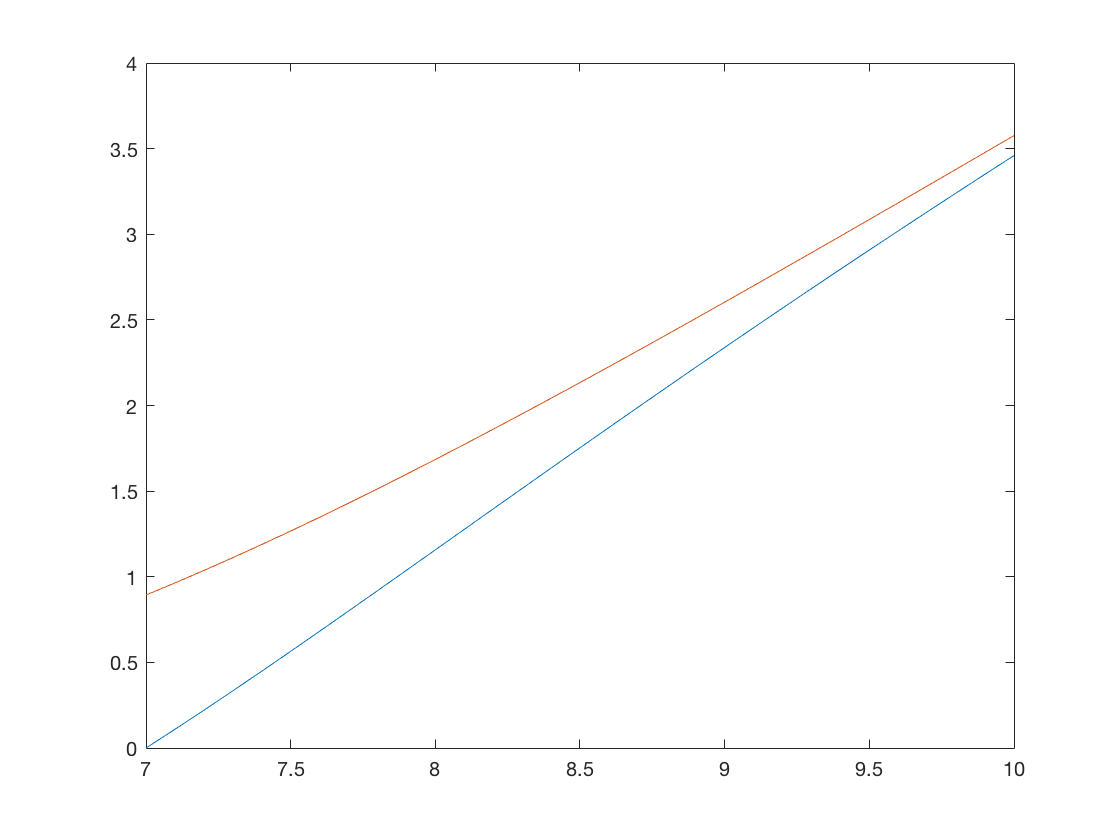
\includegraphics[scale=0.3]{A1_1_plot.png}
	\caption{Prices of down-and-out and vanilla call option against current underlier price}
\end{figure}

\subsection{Comments on plot of computation errors using BTM against theoretical values}

\begin{figure}[h]
	\centering
	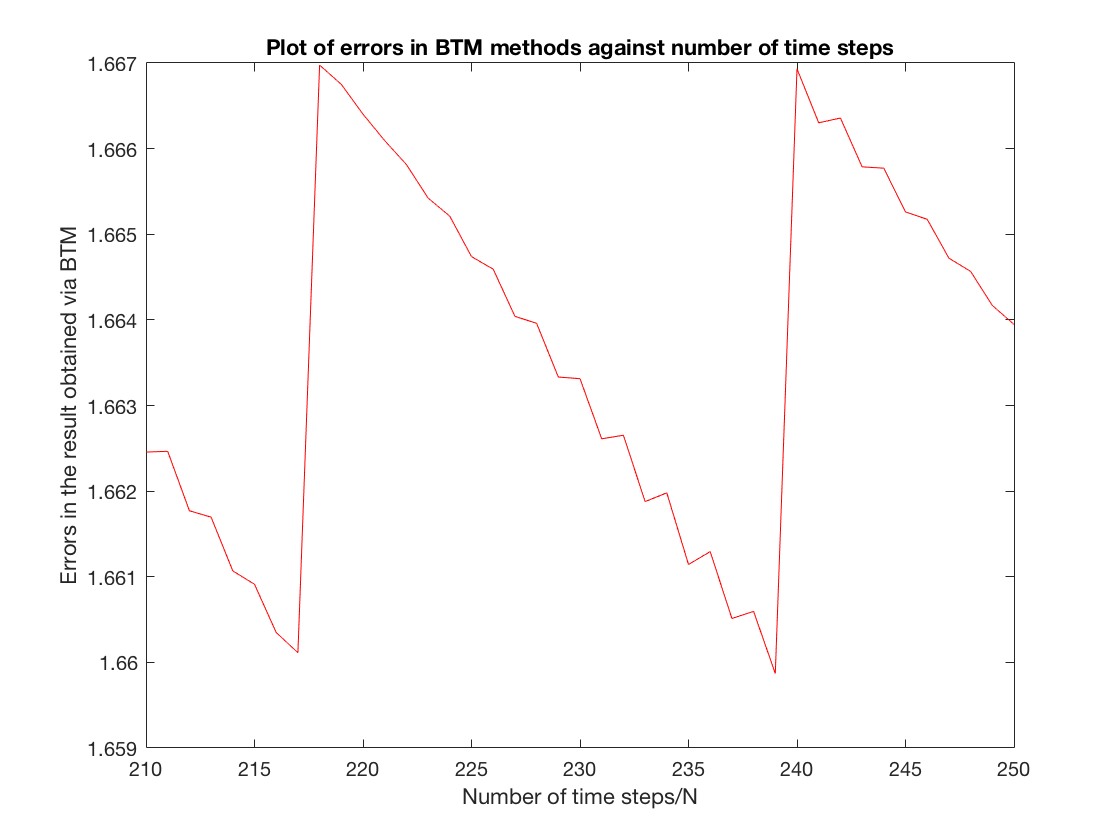
\includegraphics[scale=0.3]{A1_4_plot.PNG}
	\caption{Prices of European down-and-out call against number of time steps}
\end{figure}

\newpage

\section{European floating strike lookback put option}
\subsection*{Statement of the problem}
Write a Matlab function that implements version 1 of the single-state variable binomial tree method for approximating prices of a European floating strike lookback put option (newly issued) with $0.5$ year to maturity, current underlying price of \$1, volatility of $40\%$, dividend yield of $2\%$ and risk free rate of $4\%$. Obtain option value estiamtes for number of time steps $N$ being $200$ to $20000$ in increments of $200$. Obtain a graph of these option values versus $N$.\\
Write also a Matlab function to price European floating strike lookback put option (not newly issued). Test with same parameters with running max of \$$1.3$.

\subsection{Newly issued European floating strike lookback put options}
For the floating strike type of lookback options, we can change from a two-state model to single-state model. We make use of this property $V(A_{t},S_{t},t) = S_{t}V(\frac{A_{t}}{S_{t}}, 1, t)$, and use the new symbol $x_{t} = \ln(\frac{A_{t}}{S_{t}})$ to represent the current state on the binomial tree. Value of the option can thus be represented by $W(x_{t}, t) = \frac{V(exp(x_{t}), 1, t)}{S_{t}}$.\\
Since in this case we are only interested in the $A_{t}$ being the maximum value of underlying over time, the binomial updates of $A_{t}$ can be simplied as:
\begin{equation}
  A_{t}=
  \begin{cases}
    A_{t-1}, & \text{if}\ S_{t} = dS_{t-1} \\
    \max(A_{t-1}, S_{t}), & \text{otherwise}
  \end{cases}
\end{equation}
Furthermore, we use this upon the binomial updates of $x_{t}$:
\begin{equation}
  x_{n}^{k}=
  \begin{cases}
    x_{n-1}^{\frac{k+1}{2}} + {^{\Delta}x}, & \text{if}\ k \text{ is odd} \\
    \max(x_{n-1}^{\frac{k}{2}} - {^{\Delta}x}, 0), & \text{otherwise}
  \end{cases}
\end{equation}
where ${^{\Delta}x} = \sigma \sqrt{^{\Delta}t}$
The binomial update equation for $W(x_{n}^{k}, t_{n})$ is:
$$ W(x_{n}^{k}, t_{n}) = \exp(-r{^{\Delta}t})[puW(x_{n+1}^{2k}, t_{n+1}) + (1-p)dW(x_{n+1}^{2k+1}, t_{n+1})] $$
\begin{algorithm}[H]
 \KwData{$r, \sigma, S_{0}, \tau, N, q$}
 \KwResult{$p_{0}$, Option Premium}
 Initialization\;
 $N = \frac{T}{\delta t}$\;
 $x_{n}^{k} = k{^{\Delta}x}$\;
 Set the boundary conditions\;
 \For {i = $\max(j-N, 0)$ \dots $j+N+1$} {
  $W_{N}^{i} = \exp(x_{N}^{i}) - 1$\;
 }
 \For {n = N-1, N-2, \dots 0} {
  \If {$j - n \le 0$} {
    $W_{n}^{0} = exp(-r{^{\Delta}t})[puW_{n+1}^{0}+(1-p)dW_{n+1}^{1}]$\;
  }
  \For {k = $\max(j-n,1), \dots, j + n + 1$} {
    $W_{n}^{k} = exp(-r{^{\Delta}t})[puW_{n+1}^{k-1}+(1-p)dW_{n+1}^{k+1}]$\;
  }
 }
 $p_{0} = S_{0}W_{0}^{0}$\;
\caption{Algorithm for pricing newly issued floating strike lookback put}
\end{algorithm}
\newpage

\subsection{Previously issued European floating strike lookback put options}
In the previous case we could take advantage of the characteristic of lookback option in which all the maximum values correspond to the potential stock prices in the binomial tree. However in this case, since the option is not newly issued and we may have a previous running max which does not correspond to any of the potential stock prices, we cannot use the single state variable to fully represent both the current stock price and the running max. Therefore the following adjustment is needed:
\begin{itemize}
	\item Compare $\tilde{A}$ and $S_{0}$, if $\tilde{A}$ is smaller, treat this like a newly issued lookback option and use the previous case's algorithm
	\item let $x_{0} = \ln \frac{\tilde{A}}{S_{0}}$
	\item Determine for an integer $j$ such that $j{^{\Delta}x} < x_{0} < (j+1){^{\Delta}x}$
	\item Grow two separate linear trees from $x_{0}^{j}$ and $x_{0}^{j+1}$
	\item Perform the backward time binomial updates
	\item Interpolate between two option values at the roots to obtain option premium
\end{itemize}
Below is an algorithm developed based on this idea:\\
\begin{algorithm}[H]
 \KwData{$r, \sigma, S_{0}, \tau, N, q, \tilde{A}$}
 \KwResult{$p_{0}$, Option Premium}
 Initialization\;
 let $x_{0} = \ln \frac{\tilde{A}}{S_{0}}$ be the initial  of the single state\;
 Choose integer $j$ such that $j{^{\Delta}x} < x_{0} < (j+1){^{\Delta}x}$\;
 $N = \frac{T}{\delta t}$\;
 Set the boundary conditions\;
 \For {i = $\max(j-N, 0)$ \dots $j+N+1$} {
  $W_{N}^{i} = \exp(x_{N}^{i}) - 1$\;
 }
 \For {n = N-1, N-2, \dots 0} {
  \If {$j - n \le 0$} {
    $W_{n}^{0} = exp(-r{^{\Delta}t})[puW_{n+1}^{0}+(1-p)dW_{n+1}^{1}]$\;
  }
  \For {k = $\max(j-n,1), \dots, j + n + 1$} {
    $W_{n}^{k} = exp(-r{^{\Delta}t})[puW_{n+1}^{k-1}+(1-p)dW_{n+1}^{k+1}]$\;
  }
 }
 $p_{0}$ is approximated by interpolating between $S_{0}W_{0}^{j}$ and $S_{0}W_{0}^{j+1}$\;
\caption{Algorithm for pricing not newly issued floating strike lookback put}
\end{algorithm}
\newpage

\subsection{Analyze, compare and comment on the results}
From Figure 3, we can easily observe that as the number of time steps used in the binomial tree method slowly increases from $200$ to $20000$, the prices obtained for the newly issued floating strike lookback put option monotonically increases from \$$0.226$ to \$$0.2364$. The rate of increase gradually drops as the price increases, and we see this as an indication that the price obtained is converging to the true value of the option.\\[4mm]
\begin{figure}[h]
	\centering
	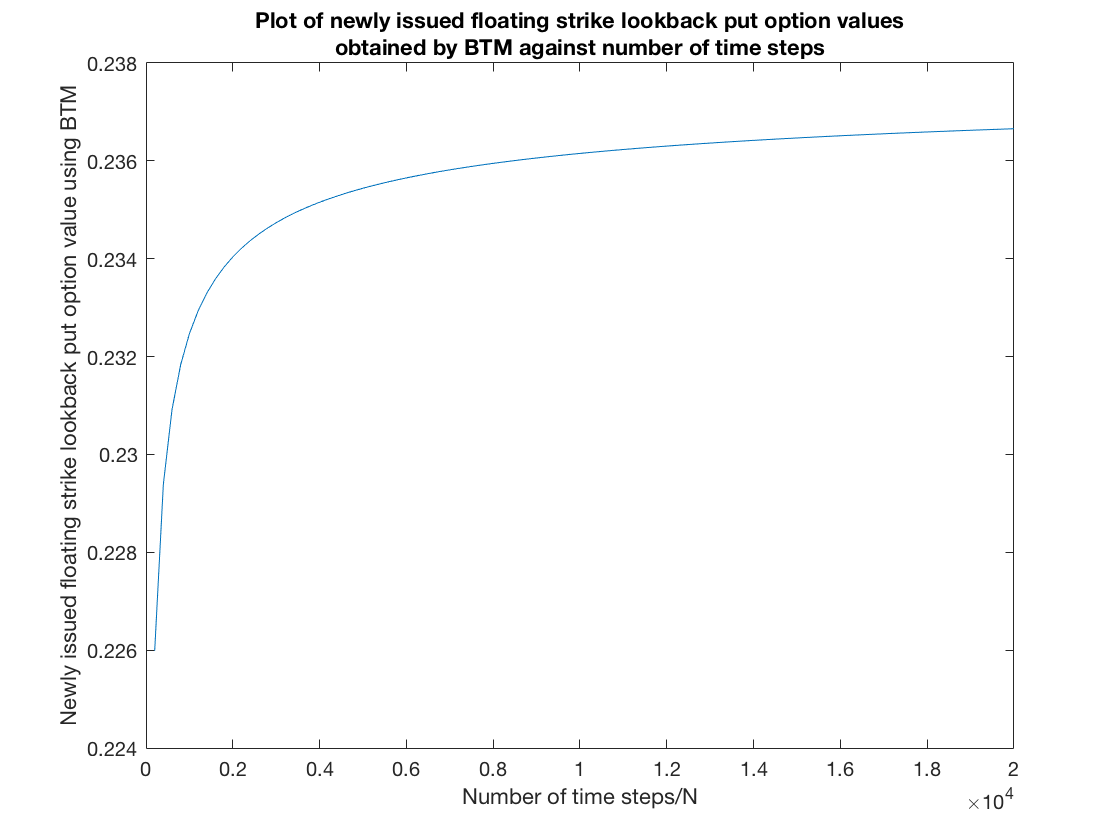
\includegraphics[scale=0.3]{A2_ni.PNG}
	\caption{Prices of newly issued floating strike lookback put against the number of time steps}
\end{figure}
If the true value is actually around $0.2364$, we should be confident that the binomial tree method with single-state modification for the European floating strike lookback put option can almost always give a good estimate of the price since the initially computed price with only $200$ time steps is very close to the true value. However, the closed-form formula does not exist for this case but once we have the finite different equations for the lookback options, the prices from FDM can be used to cross-validate the ones from binomial tree methods.\\[4mm]
Similar to the newly issued lookback put options, the prices of the previously issued lookback puts also tend from around \$$0.3466$ to \$$0.3513$, as shown in figure 4. The increase in price is also montonic and the rate of increase drops as the price increases. If we make the same assumption as for the newly issued puts, i.e. the true value lies around \$$0.3513$, we should be able to observe that value obtained from merely $200$ time steps binomial tree method is at \$$0.3466$ with only difference of \$$0.05$ from the true value.\\[4mm]
A natural question to ask may be: is this an indication that the binomial tree method may give us even more accurate value for a previously issued lookback put option? However, we shall notice that this may only attribute to the fact of having a relatively large previous running max.\\[4mm]
\begin{figure}[h]
	\centering
	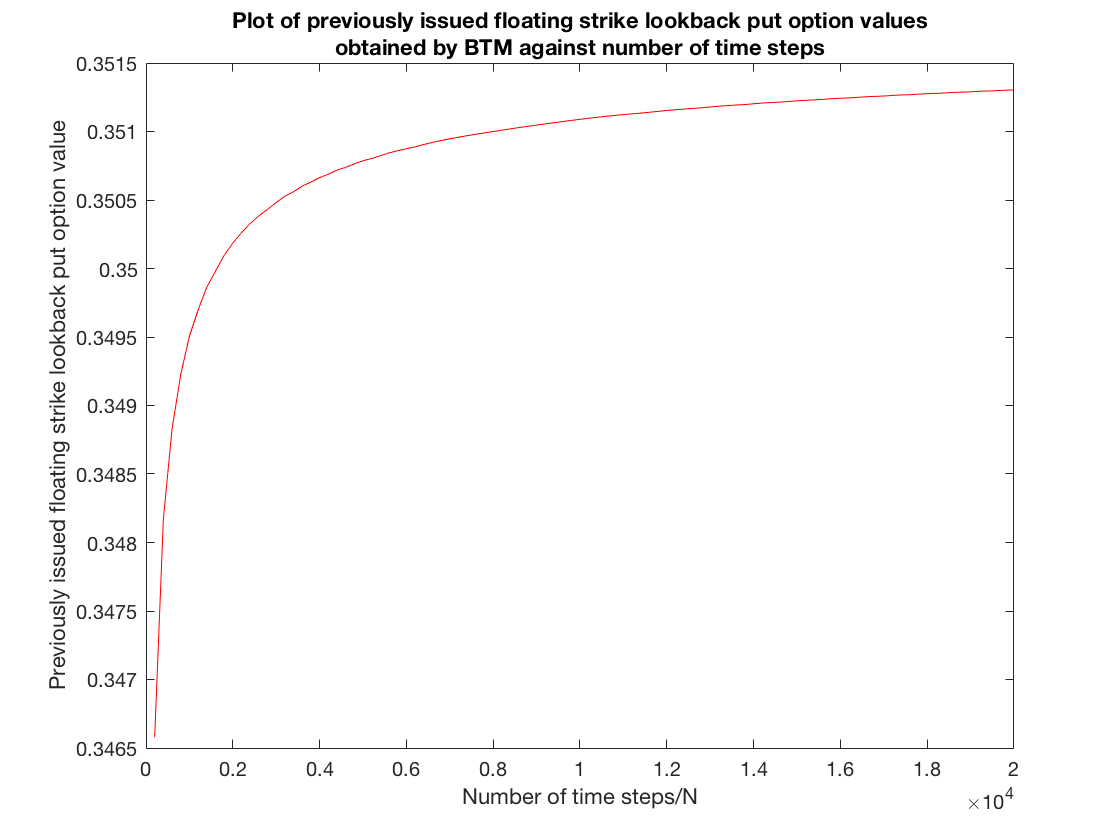
\includegraphics[scale=0.3]{A2_pi.PNG}
	\caption{Prices of previously issued floating strike lookback put against the number of time steps}
\end{figure}
We should then plot them on the same diagram and it is not hard to observe that the two price curves of these two options are very similar. Although their price levels are very different, the curvatures at various time points of the price curves are similar.
\begin{figure}[h]
	\centering
	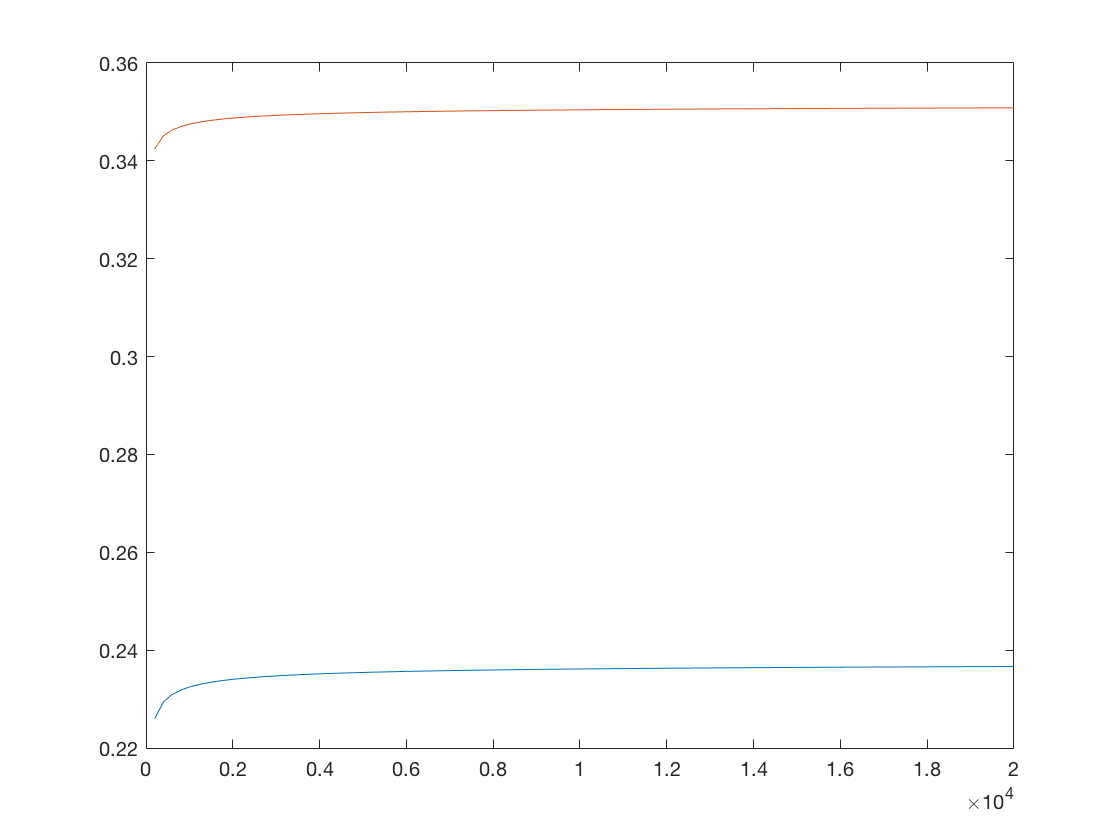
\includegraphics[scale=0.3]{A2.PNG}
	\caption{Prices of not newly issued floating strike lookback put against the number of time steps}
\end{figure}

\end{document}